\newcommand\mybox[2][]{\tikz[overlay]\node[fill=lightyellow,inner sep=2pt, anchor=text, rectangle, rounded corners=1mm,draw=black,#1] {#2};\phantom{#2}}

\tikzstyle{reddot}=[draw=black,line width=1pt,minimum size=1.5mm,inner sep=0pt,outer sep=0pt,shape=circle,fill=blue]
\tikzstyle{bluedot}=[draw=blue,minimum size=0.5mm,inner sep=0pt,outer sep=0pt,shape=circle,fill=blue]

%%%%%%%%%%%%%%%%%%%%%%%%%%%%%%%%%%%%%%%%%%%%%%%%%%%%%%%%%%%%%%%%%%%%%%%%%%%%%%%%
\begin{frame}{The intrinsic dimension of data}

\begin{itemize}
\item
modern learning algorithms use high dimensional data

\item
\textbf{curse of dimensionality:}
\textcolor{red}{
the runtime of nearest neighbor queries grows exponentially with the dimension of data
}

\pause
\item
\textbf{manifold hypothesis:}
\textcolor{darkgreen}{
real world datasets are low dimensional manifolds embedded in high dimensional spaces
}
\end{itemize}

%Example:

\pause
\begin{center}
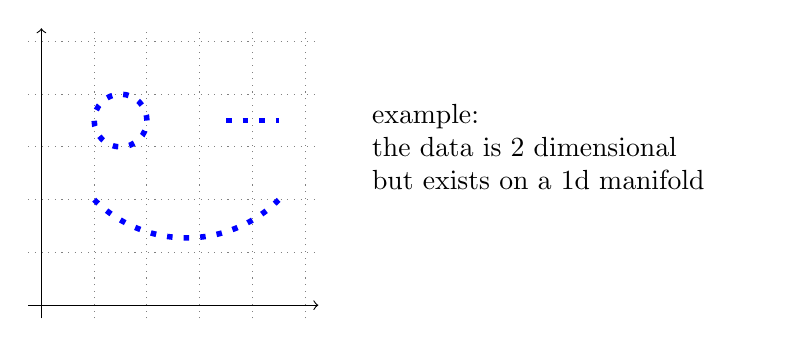
\begin{tikzpicture}[scale=0.67]
% draw the grid
\draw[->] (0,-0.25) -- (0,5.25) ;
\draw[->] (-0.25,0) -- (5.25,0) ;
\foreach \i in {1,...,5} {
    \draw[dotted,draw=gray] (-0.25,\i) -- (5.25,\i);
}
\foreach \i in {1,...,5} {
    \draw[dotted,draw=gray] (\i,-0.25) -- (\i,5.25);
}

\draw[loosely dotted,draw=blue,line width=2pt] (1,2) to[in=225,out=-45] (4.5,2);
\path[loosely dotted,draw=blue,line width=2pt] (1.5,3.5) circle (0.5);
\draw[loosely dotted,draw=blue,line width=2pt] (3.5,3.5) to (4.5,3.5);

\node[text width=5cm] at (10,3) {example: \\ the data is 2 dimensional \\ but exists on a 1d manifold};

\end{tikzpicture}
\end{center}

\end{frame}

%%%%%%%%%%%%%%%%%%%%%%%%%%%%%%%%%%%%%%%%%%%%%%%%%%%%%%%%%%%%%%%%%%%%%%%%%%%%%%%%

\begin{frame}{The intrinsic dimensions: \mybox{$\cexp$}, $\cdoub$, and $\chole$}

The \textbf{expansion constant} is defined as:
$$
\cexp = \max_{x\in X, \delta\ge0} \left\{
    \frac{|B(x,2\delta)|}{|B(x,\delta)|}
      \right\}
$$
\vspace{-0.1in}
where
$$
B(x,\delta) = \{x' \in X : d(x,x') \le \delta \}
$$
%is the ball of radius $\delta$ centered at point $x$.

\vspace{0.1in}
\hrule
\vspace{0.1in}
%%%%%%%%%%%%%%%%%%%%%%%%%%%%%%%%%%%%%%%%

\begin{tikzpicture}[scale=0.67]
% draw the grid
\draw[->] (0,-0.25) -- (0,5.25) ;
\draw[->] (-0.25,0) -- (5.25,0) ;
\foreach \i in {1,...,5} {
    \draw[dotted,draw=gray] (-0.25,\i) -- (5.25,\i);
}
\foreach \i in {1,...,5} {
    \draw[dotted,draw=gray] (\i,-0.25) -- (\i,5.25);
}

%\foreach \i in {1,...,10} {
    %\foreach \j in {1,...,10} {
        %\node[bluedot] at (0.3*\i,0.3*\j) {};
    %}
%}
\node[bluedot] at (2.5,2.5) {};
\foreach \i in {1,...,10} {
    \node[bluedot] at (2.5+0.2*\i,2.5-0.2*\i) {};
    \node[bluedot] at (2.5-0.2*\i,2.5+0.2*\i) {};
}

\uncover<2-5> {
\node[reddot] at (2.5,2.5) {};
\path[draw=black] (2.5,2.5) circle (1.4);
\path[draw=black] (2.5,2.5) circle (2.85);
}

\uncover<2-5> {
\node[fill=white] at (1.5,0) {\textcolor{darkgreen}{robust}};
\node at (2.5,-1) {\textcolor{darkgreen}{$\log\cexp=O(d)$}} ;
}
\end{tikzpicture}
%%%%%%%%%%%%%%%%%%%%
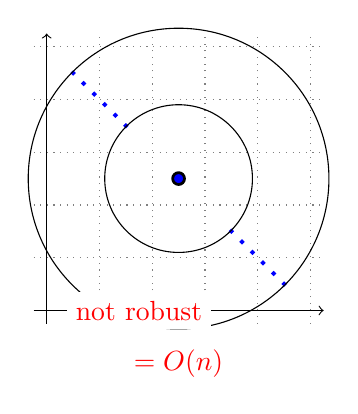
\begin{tikzpicture}[scale=0.67]
% draw the grid
\draw[->] (0,-0.25) -- (0,5.25) ;
\draw[->] (-0.25,0) -- (5.25,0) ;
\foreach \i in {1,...,5} {
    \draw[dotted,draw=gray] (-0.25,\i) -- (5.25,\i);
}
\foreach \i in {1,...,5} {
    \draw[dotted,draw=gray] (\i,-0.25) -- (\i,5.25);
}

\node[bluedot] at (2.5,2.5) {};
\foreach \i in {1,...,6} {
    \node[bluedot] at (3.3+0.2*\i,1.7-0.2*\i) {};
    \node[bluedot] at (1.7-0.2*\i,3.3+0.2*\i) {};
}

\uncover<3-5>{
\node[reddot] at (2.5,2.5) {};
\path[draw=black] (2.5,2.5) circle (1.4);
\path[draw=black] (2.5,2.5) circle (2.85);
}
\uncover<3-5> {
\node[fill=white] at (1.75,0) {\textcolor{red}{not robust}};
\node at (2.5,-1) {\textcolor{red}{$\cexp=O(n)$}} ;
}
\end{tikzpicture}
%%%%%%%%%%%%%%%%%%%%
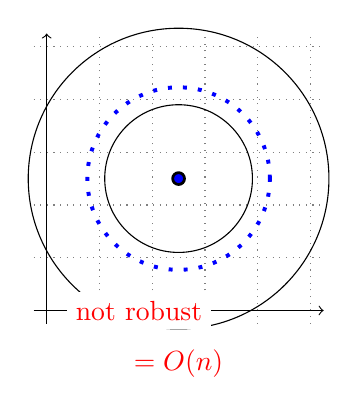
\begin{tikzpicture}[scale=0.67]
% draw the grid
\draw[->] (0,-0.25) -- (0,5.25) ;
\draw[->] (-0.25,0) -- (5.25,0) ;
\foreach \i in {1,...,5} {
    \draw[dotted,draw=gray] (-0.25,\i) -- (5.25,\i);
}
\foreach \i in {1,...,5} {
    \draw[dotted,draw=gray] (\i,-0.25) -- (\i,5.25);
}

\node[bluedot] at (2.5,2.5) {};
\path[loosely dotted,draw=blue,line width=0.5mm] (2.5,2.5) circle (1.73);

\uncover<4-5>{
\node[reddot] at (2.5,2.5) {};
\path[draw=black] (2.5,2.5) circle (1.4);
\path[draw=black] (2.5,2.5) circle (2.85);
}
\uncover<4-5>   {
    \node[fill=white] at (1.75,0) {\textcolor{red}{not robust}};
    \node at (2.5,-1) {\textcolor{red}{$\cexp=O(n)$}};
}
\end{tikzpicture}

%%%%%%%%%%%%%%%%%%%%

\uncover<5>{
\vspace{-2.85in}
\begin{tikzpicture}
\node[fill=lightyellow,draw=black,thick,text width=11.05cm,rounded corners=0.1cm,inner sep=0.2in] at (0,0) { 
    \textcolor{darkgreen}{Advantage: suitable for exact nearest neighbor queries}
    \\
    \textcolor{red}{Disadvantage: not robust to changes in the data set}
    %\textcolor{red}{Disadvantage: cannot be used for exact nearest neighbor queries}
};
\end{tikzpicture}
}

\vspace{1.8in}

\end{frame}

%%%%%%%%%%%%%%%%%%%%%%%%%%%%%%%%%%%%%%%%%%%%%%%%%%%%%%%%%%%%%%%%%%%%%%%%%%%%%%%%

\begin{frame}{The intrinsic dimensions: $\cexp$, \mybox{$\cdoub$}, and $\chole$}

A set $C$ is a \textbf{$\delta$-covering} of $X$ if for all $x\in X$, there exists a $c \in C$ such that $\dist{x}{c} \le \delta$.
The \textbf{covering number} of $X$, denoted $N_\delta(X)$, is the cardinality of the smallest $\delta$-covering.
The \textbf{doubling constant} is 
\begin{equation}
\cdoub = \max_{x\in X,\delta>0} N_\delta( B(x,2\delta))
.
\end{equation}

%
%An \textbf{$r$-covering} of a set $X$ is a subset of $X$ such that all pairwise distances are greater than $r$. %$\{x_1,x_2,...x_M\} \subset X$ such that $\dist{x_i}{x_j} > r$ for all distinct $i,j$.
%
%The \textbf{$r$-packing number} $M_r (X)$ is the cardinality of the largest $r$-packing.
%

\vspace{0.1in}
\hrule
\vspace{0.1in}
%%%%%%%%%%%%%%%%%%%%%%%%%%%%%%%%%%%%%%%%

\begin{tikzpicture}[scale=0.67]
% draw the grid
\draw[->] (0,-0.25) -- (0,5.25) ;
\draw[->] (-0.25,0) -- (5.25,0) ;
\foreach \i in {1,...,5} {
    \draw[dotted,draw=gray] (-0.25,\i) -- (5.25,\i);
}
\foreach \i in {1,...,5} {
    \draw[dotted,draw=gray] (\i,-0.25) -- (\i,5.25);
}

%\foreach \i in {1,...,10} {
    %\foreach \j in {1,...,10} {
        %\node[bluedot] at (0.3*\i,0.3*\j) {};
    %}
%}
\node[bluedot] at (2.5,2.5) {};
\foreach \i in {1,...,10} {
    \node[bluedot] at (2.5+0.2*\i,2.5-0.2*\i) {};
    \node[bluedot] at (2.5-0.2*\i,2.5+0.2*\i) {};
}

\uncover<2-5> {
\node[reddot]  at (2.5,2.5) {};
\path[draw=black] (2.5,2.5) circle (1.4);
\path[draw=black] (2.5,2.5) circle (2.85);

\node[reddot]  at (1.3,3.7) {};
\path[draw=black] (1.3,3.7) circle (1.4);
\node[reddot]  at (3.7,1.3) {};
\path[draw=black] (3.7,1.3) circle (1.4);
}

\uncover<2-5> {
\node[fill=white] at (1.5,0) {\textcolor{darkgreen}{robust}};
\node at (2.5,-1) {\textcolor{darkgreen}{$\log\cdoub=O(d)$}} ;
}
\end{tikzpicture}
%%%%%%%%%%%%%%%%%%%%
\begin{tikzpicture}[scale=0.67]
% draw the grid
\draw[->] (0,-0.25) -- (0,5.25) ;
\draw[->] (-0.25,0) -- (5.25,0) ;
\foreach \i in {1,...,5} {
    \draw[dotted,draw=gray] (-0.25,\i) -- (5.25,\i);
}
\foreach \i in {1,...,5} {
    \draw[dotted,draw=gray] (\i,-0.25) -- (\i,5.25);
}

\node[bluedot] at (2.5,2.5) {};
\foreach \i in {1,...,6} {
    \node[bluedot] at (3.3+0.2*\i,1.7-0.2*\i) {};
    \node[bluedot] at (1.7-0.2*\i,3.3+0.2*\i) {};
}

\uncover<3-5>{
\node[reddot] at (2.5,2.5) {};
\path[draw=black] (2.5,2.5) circle (1.4);
\path[draw=black] (2.5,2.5) circle (2.85);

\node[reddot]  at (1.3,3.7) {};
\path[draw=black] (1.3,3.7) circle (1.4);
\node[reddot]  at (3.7,1.3) {};
\path[draw=black] (3.7,1.3) circle (1.4);
}
\uncover<3-5> {
\node[fill=white] at (1.5,0) {\textcolor{darkgreen}{robust}};
\node at (2.5,-1) {\textcolor{darkgreen}{$\log\cdoub=O(d)$}} ;
}
\end{tikzpicture}
%%%%%%%%%%%%%%%%%%%%
\begin{tikzpicture}[scale=0.67]
% draw the grid
\draw[->] (0,-0.25) -- (0,5.25) ;
\draw[->] (-0.25,0) -- (5.25,0) ;
\foreach \i in {1,...,5} {
    \draw[dotted,draw=gray] (-0.25,\i) -- (5.25,\i);
}
\foreach \i in {1,...,5} {
    \draw[dotted,draw=gray] (\i,-0.25) -- (\i,5.25);
}

\node[bluedot] at (2.5,2.5) {};
\path[loosely dotted,draw=blue,line width=0.5mm] (2.5,2.5) circle (1.73);

\uncover<4-5>{
\node[reddot] at (2.5,2.5) {};
\path[draw=black] (2.5,2.5) circle (1.4);
\path[draw=black] (2.5,2.5) circle (2.85);
}
\uncover<4-5>   {
\node[reddot]  at (1.3,3.7) {};
\path[draw=black] (1.3,3.7) circle (1.4);
\node[reddot]  at (3.7,3.7) {};
\path[draw=black] (3.7,3.7) circle (1.4);
\node[reddot]  at (3.7,1.3) {};
\path[draw=black] (3.7,1.3) circle (1.4);
\node[reddot]  at (1.3,1.3) {};
\path[draw=black] (1.3,1.3) circle (1.4);

    \node[fill=white] at (1.5,0) {\textcolor{darkgreen}{robust}};
    \node at (2.5,-1) {\textcolor{darkgreen}{$\log\cdoub=O(d)$}};
}
\end{tikzpicture}

\uncover<5>{
\vspace{-2.80in}
\begin{tikzpicture}
\node[fill=lightyellow,draw=black,thick,text width=11.05cm,rounded corners=0.1cm,inner sep=0.2in] at (0,0) { 
    \textcolor{darkgreen}{Advantage: robust to all changes in the data set}
    \\
    \textcolor{red}{Disadvantage: cannot be used for exact nearest neighbor queries}
};
\end{tikzpicture}
}

\vspace{1.8in}

\end{frame}

%%%%%%%%%%%%%%%%%%%%%%%%%%%%%%%%%%%%%%%%%%%%%%%%%%%%%%%%%%%%%%%%%%%%%%%%%%%%%%%%

\begin{frame}{The intrinsic dimensions: $\cexp$, $\cdoub$, and \mybox{$\chole$}}

%A set $C$ is a \textbf{$\delta$-covering} of $X$ if for all $x\in X$, there exists a $c \in C$ such that $\dist{x}{c} \le \delta$.
%The \textbf{covering number} of $X$, denoted $M_\delta(X)$, is the cardinality of the largest $\delta$-covering.
%The \textbf{doubling constant} is 
%\begin{equation}
%\cdoub = \max_{x\in X,\delta>0} M_\delta( B(x,2\delta))
%.
%\end{equation}
The \textbf{hole dimension} is like the doubling dimension,
but ignores a hole removed from the center of the enclosing ball.
It is defined as
\begin{align}
    \label{eq:chole}
    \chole
    = 
    &\max_{x\in X, \epsilon \ge 0, \delta > 0} 
    N_\delta\big( B(x,\epsilon+2\delta) \setminus B(x,\epsilon) \big)
    \\
    &
    ~~~~~~\text{s.t.}
    ~~
    %B(x,\epsilon+\delta) \setminus B(x,\delta) = \{\}
    B(x,\epsilon) = \{x\}
    .
\end{align}

%
%An \textbf{$r$-covering} of a set $X$ is a subset of $X$ such that all pairwise distances are greater than $r$. %$\{x_1,x_2,...x_M\} \subset X$ such that $\dist{x_i}{x_j} > r$ for all distinct $i,j$.
%
%The \textbf{$r$-packing number} $M_r (X)$ is the cardinality of the largest $r$-packing.
%

\vspace{0.1in}
\hrule
\vspace{0.1in}
%%%%%%%%%%%%%%%%%%%%%%%%%%%%%%%%%%%%%%%%

\begin{tikzpicture}[scale=0.67]
% draw the grid
\draw[->] (0,-0.25) -- (0,5.25) ;
\draw[->] (-0.25,0) -- (5.25,0) ;
\foreach \i in {1,...,5} {
    \draw[dotted,draw=gray] (-0.25,\i) -- (5.25,\i);
}
\foreach \i in {1,...,5} {
    \draw[dotted,draw=gray] (\i,-0.25) -- (\i,5.25);
}

%\foreach \i in {1,...,10} {
    %\foreach \j in {1,...,10} {
        %\node[bluedot] at (0.3*\i,0.3*\j) {};
    %}
%}
\node[bluedot] at (2.5,2.5) {};
\foreach \i in {1,...,9} {
    \node[bluedot] at (2.5+0.2*\i,2.5-0.2*\i) {};
    \node[bluedot] at (2.5-0.2*\i,2.5+0.2*\i) {};
}

\uncover<6-9> {
%\node[reddot]  at (2.5,2.5) {};
\path[draw=black] (2.5,2.5) circle (0.2);
\path[draw=black] (2.5,2.5) circle (2.6);

\path[draw=lightgray,opacity=0.5,line width=1.6cm] (2.5,2.5) circle (1.4);

\node[reddot]  at (1.5,3.5) {};
\path[draw=black] (1.5,3.5) circle (1.2);
\node[reddot]  at (3.5,1.5) {};
\path[draw=black] (3.5,1.5) circle (1.2);
}

\uncover<6-9> {
\node[fill=white] at (1.5,0) {\textcolor{darkgreen}{robust}};
\node at (2.5,-1) {\textcolor{darkgreen}{$\log\chole=O(d)$}} ;
}
\end{tikzpicture}
%%%%%%%%%%%%%%%%%%%%
\begin{tikzpicture}[scale=0.67]
% draw the grid
\draw[->] (0,-0.25) -- (0,5.25) ;
\draw[->] (-0.25,0) -- (5.25,0) ;
\foreach \i in {1,...,5} {
    \draw[dotted,draw=gray] (-0.25,\i) -- (5.25,\i);
}
\foreach \i in {1,...,5} {
    \draw[dotted,draw=gray] (\i,-0.25) -- (\i,5.25);
}

\node[bluedot] at (2.5,2.5) {};
\foreach \i in {1,...,5} {
    \node[bluedot] at (3.3+0.2*\i,1.7-0.2*\i) {};
    \node[bluedot] at (1.7-0.2*\i,3.3+0.2*\i) {};
}

\uncover<2-9> {
    \node[reddot]  at (2.5,2.5) {};
    \path[draw=black] (2.5,2.5) circle (1.35);
    \draw (2.5,2.5) -- node[above] {$\epsilon$} (3.85,2.5);
}
\uncover<3-9> {
    \path[draw=black] (2.5,2.5) circle (2.65);
    \path[draw=lightgray,opacity=0.5,line width=0.85cm] (2.5,2.5) circle (2);
    \draw (3.455,3.455) --  (4.365,4.365);
    \node at (3.75,4.25) {\small $2\delta$};
}
\uncover<4-9> {
    \node[reddot]  at (1.1,3.9) {};
    \path[draw=black] (1.1,3.9) circle (0.65);
    \node[reddot]  at (3.9,1.1) {};
    \path[draw=black] (3.9,1.1) circle (0.65);

    \draw(3.9,1.1) -- (4.4,1.6);
    \node at (4.0,1.5) {\small $\delta$};
}
\uncover<5-9> {
\node[fill=white] at (1.5,0) {\textcolor{darkgreen}{robust}};
\node at (2.5,-1) {\textcolor{darkgreen}{$\log\chole=O(d)$}} ;
}
\end{tikzpicture}
%%%%%%%%%%%%%%%%%%%%
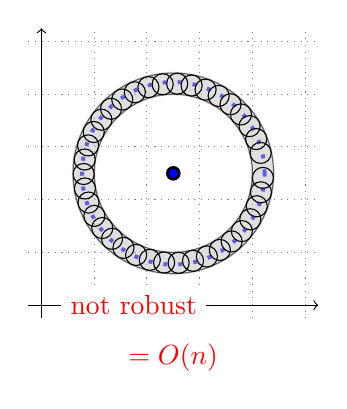
\begin{tikzpicture}[scale=0.67]
% draw the grid
\draw[->] (0,-0.25) -- (0,5.25) ;
\draw[->] (-0.25,0) -- (5.25,0) ;
\foreach \i in {1,...,5} {
    \draw[dotted,draw=gray] (-0.25,\i) -- (5.25,\i);
}
\foreach \i in {1,...,5} {
    \draw[dotted,draw=gray] (\i,-0.25) -- (\i,5.25);
}

\node[bluedot] at (2.5,2.5) {};
\path[loosely dotted,draw=blue,line width=0.5mm] (2.5,2.5) circle (1.73);

\uncover<8-9>{
    \node[reddot] at (2.5,2.5) {};
    \path[draw=black] (2.5,2.5) circle (1.5);
    \path[draw=black] (2.5,2.5) circle (1.9);
    \path[draw=lightgray,opacity=0.5,line width=0.3cm] (2.5,2.5) circle (1.7);
}
    %\foreach \i in {1,...,20) {
        %\path[draw=black] (1.3*\i,1.3*\i) circle (0.2);
    %}
\uncover<8-9>   {
    \foreach \i in {10,...,47} {
        \path[draw=black] ({2.5+1.7*sin(\i/pi*29.2)} ,{2.5+1.7*cos(\i/pi*29.2)} ) circle (0.2);
        %\draw[dotted,draw=lightgray] (\i,-0.25) -- (\i,5.25);
    }
    %\path[draw=black] (1.3,3.7) circle (0.2);
    %\path[draw=black] (3.7,3.7) circle (0.2);
    %\path[draw=black] (3.7,1.3) circle (0.2);

    \node[fill=white] at (1.75,0) {\textcolor{red}{not robust}};
    \node at (2.5,-1) {\textcolor{red}{$\chole=O(n)$}};
}
\end{tikzpicture}

\uncover<9>{
\vspace{-2.85in}
\begin{tikzpicture}
\node[fill=lightyellow,draw=black,thick,text width=11.05cm,rounded corners=0.1cm,inner sep=0.2in] at (0,0) { 
    \textcolor{darkgreen}{Advantage: more robust than the expansion dimension $\cexp$}
    \\
    \textcolor{darkgreen}{Advantage: suitable for exact nearest neighbor queries} 
    %\textcolor{red}{Disadvantage: cannot be used for exact nearest neighbor queries}
};
\end{tikzpicture}
}

\vspace{1.8in}

\end{frame}

%%%%%%%%%%%%%%%%%%%%%%%%%%%%%%%%%%%%%%%%%%%%%%%%%%%%%%%%%%%%%%%%%%%%%%%%%%%%%%%%
